\normaltrue \difficilefalse \tdifficilefalse
\correctionfalse

%\UPSTIidClasse{11} % 11 sup, 12 spé
%\newcommand{\UPSTIidClasse}{12}

\exer{Barrière Sympact $\star$ \label{C2:09:14}}
\setcounter{question}{0}\UPSTIcompetence[2]{C2-09}
\index{Compétence C2-09}
\index{TEC}
\index{Théorème de l'énergie cinétique}
\index{Barrière Sympact}
\index{Croix de Malte}
\ifcorrection
\else
\marginnote{\textbf{Pas de corrigé pour cet exercice.}}
\fi

\ifprof
\else
Soit le mécanisme suivant. On a $\vect{AC}=H\vect{j_0}$ et $\vect{CB}=R\vect{i_1}$. De plus, 
$H=\SI{120}{mm}$ et $R=\SI{40}{mm}$. De plus, on note :
\begin{itemize}
\item $G_1$ le centre d'inertie du solide \textbf{1} tel que $\vect{CG_1}=\dfrac{R}{2} \vi{1}$, $m_1$ sa masse et $\inertie{G_1}{1}=\matinertie{A_1}{B_1}{C_1}{0}{0}{0}{\rep{1}}$ sa matrice d'inertie;
\item $G_2$ le centre d'inertie du solide \textbf{2} tel que $\vect{G_2}=a \vi{2}+b\vj{2}$, $m_2$ sa masse et $\inertie{G_2}{2}=\matinertie{A_2}{B_2}{C_2}{0}{0}{0}{\rep{2}}$ sa matrice d'inertie.
\end{itemize}
On note $C_m\vk{0}$ le couple moteur agissant sur le solide \textbf{1} et $C_r\vk{0}$ le couple exercé par un ressort de torsion agissant sur les solides \textbf{0} et \textbf{2}). L'accélération de la pesanteur est donnée par $\vect{g}=-g\vj{0}$.

\begin{center}
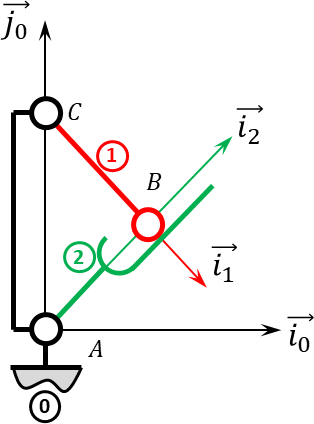
\includegraphics[width=\linewidth]{14_01}
\end{center}
\fi

On rappelle que la loi entrée sortie est donnée par la relation *** établie à l'exercice \ref{C2:06:14}.

\question{Tracer le graphe d'analyse en indiquant l'ensemble des actions mécaniques agissant sur les différents solides.}
\ifprof
\else
\fi

\question{Déterminer l'ensemble des puissances intérieures à l'ensemble \textbf{1+2}.}
\ifprof
\else
\fi

\question{Déterminer l'ensemble des puissances extérieures à l'ensemble \textbf{1+2}.}
\ifprof
\else
\fi

\question{Déterminer $\ec{1+2}{0}$.}
\ifprof
\else
\fi

\question{Déterminer la loi de mouvement en appliquant le théorème de l'énergie cinétique.}
\ifprof
\else
\fi

\ifprof
\else
\begin{flushright}
\footnotesize{Corrigé  voir \ref{C2:09:14}.}
\end{flushright}%
\fi